\chapter{Nevrologiske sykdommer}
		\section{Hva du skal ta med deg videre:}
			\begin{itemize}
				\item Husk FAST -Fjes -Arm -Språk -Tid.\\
				\item Ta et blodsukker.\\
				\item Drypp er en av de største risikofaktorene for slag.\\
				\item Slagpasienter som sliter språklig er ikke dumme.\\
				\item Regelmessig puls?\\
			\end{itemize}
		\section{Kort om denne delen...}
			Hjernen er hoveddelen av sentralnervesystemet. Det er ikke meningen å snakke om hele nervesystemet, men denne delen omhandler slag, drypp og demens som er noen av de største utfordringene vi har i dag. Jeg kommer ikke til å bruke mye pass på parkinsons og andre sykdommer da dette ville blitt for omfattende for dette dagsseminaret.
		\section{Anatomi}
			\paragraph{Et komplekst bilde}
				\begin{figure}[ht]
                      \centering
                      	\frame{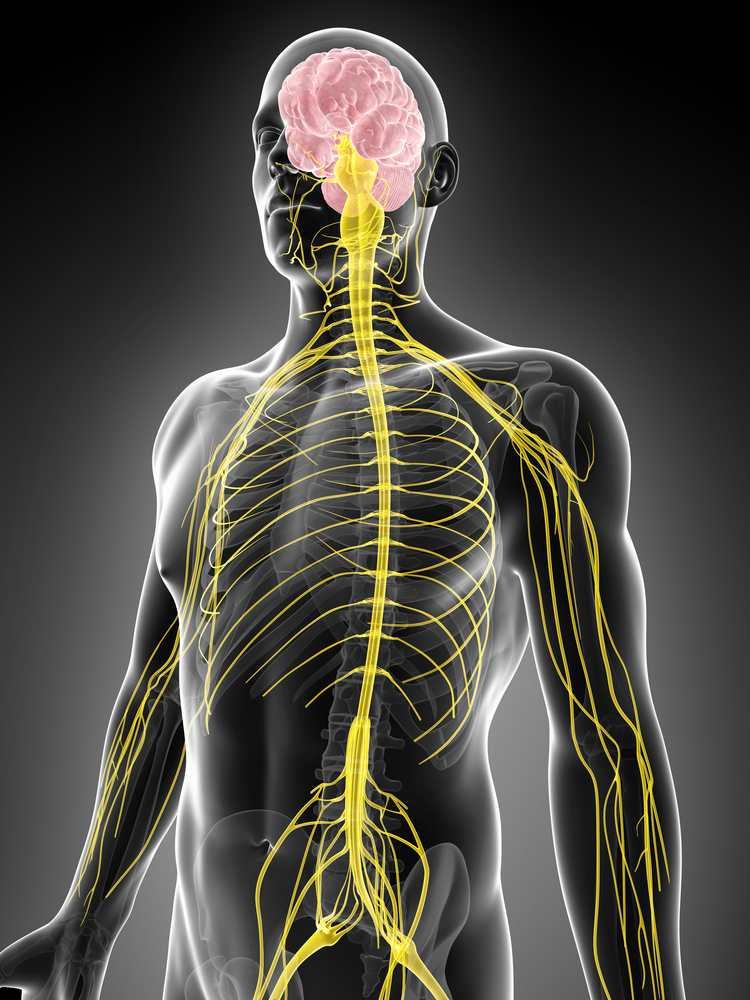
\includegraphics[width=3in]{./kap/bilder/nevro1.jpg}}%!!! må byttes ut, copyright Greys anatomy
                      \caption{Oversiktsbilde over det sentrale nervesystem}
                      %{Her ser vi et bilde som illusterer lungene og den antomiske oppbygningen}%\textit{tjenestetilbudene}.]
                    \end{figure}
			\paragraph{Inndelingen\\}
				Hjernen er forbundet med ryggmargen i medulla oblongata, eller den forlengede ryggmargen på norsk. Selve ryggmargen går omlag 2/3 ned av hele lengden av ryggen. 
		\section{Fysiologi}
			\paragraph{Kompleks struktur\\}
				Hjernen er organisert i områder som jobber med hver sine oppgaver. For eksempel sitter personligheten foran, rett bak pannen. Alle nervecellene er koblet sammen som et stort nettverk som løser hver sine oppgaver, men også jobber på kryss og tvers. 
			\paragraph{Plastisitet\\}
				En viktig egenskap er kalt "Hjernens plastisitet". Det betyr at hjernen kan reparere og til dels få tilbake tapte funksjoner igjen. for eksempel kan en person som har hatt slag trene seg opp ved å bruke en annen del av hjernen enn den som ble skadet. 	
		\section{Patologi}
			\paragraph{Sykdommer i blodårene\\}
				Som beskrevet i \nameref{sec:athero} på side \pageref{sec:athero} %!!!
				er årsaken til slag og drypp en forkalking av blodårene og en plutselig tiltetting av disse\cite{FA-athero}. Det som følger er omtrent som ved hjerteinfarkt: en del av hjernen mister oksygentilførselen og nervene dør. Ettersom hvor den tette åren sitter blir symptomene lokalisert på kroppen.
				%Homonkulus bilde!!!
			\paragraph{Sykdommer i nervescellene\\}
				Demens forårsakes av at det lagres et protein som heter tau(egentlig den greske bokstaven T), og som ødelegger nervecellene det lagres inne i. Det finnes flere typer demens og behandlingen er forskjellig. Mest kjent er Alzheimers demens. I dag er demens en sykdom som ikke har god behandling. Det finnes noen medisiner som reduserer symptomer men det er oftest kortvarig. 
		\section{Klinikk}
			\subsection{Slag og drypp}
			\subsection{Demens}
				\subsubsection{Alzheimers}
				\subsubsection{Andre former for demens}
		\section{Pasienteksempler}
			\subsection{Pasient 3}
			\subsection{Pasient 4}


\newpage